\documentclass[a4paper]{article}
\usepackage{amsthm}
\usepackage{amssymb}
\usepackage{amsbsy}
\usepackage{amsmath}
\usepackage[
  margin=1.5cm,
  includefoot,
  footskip=30pt,
]{geometry}
\usepackage{layout}
\usepackage{graphicx}
\title{Probabilistic Graphical Models : Homework 1}
\author{Raphael Avalos\\raphael@avalos.fr}
\date{10/10/18}
\graphicspath{ {./plots/} }
\begin{document}
\maketitle
\section{Formulas}
\subsection{Exercise 1}
We have $N$ samples $(x_i,y_i)$
$\pmb{\pi} = (\pi_1, ..., \pi_M), \pmb{\theta} = (\theta_{1,1}, ... \theta_{M,K})$	\\
$a_m = \mid \{ i \mid  z_i = m, \forall i \in [1,N]\}\mid $, $b_{m,k} = \mid \{ i \mid  z_i = m \text{ and } x_i = k, \forall i \in [1,N]\}\mid $
\begin{align*}
\tilde{\pi}_m &= \frac{a_m}{N} \\
\tilde{\theta}_{m,k} &= \frac{b_{m,k}}{N}
\end{align*}
Moreover $p(y=1 \mid x)$ have the same form of logistic regression.
\subsection{Exercise 2}
\subsubsection{LDA}
\begin{align*}
\tilde{\omega} &= \frac{n}{N} \\
\tilde{\mu}_0 &= \frac{1}{n} \sum_{\substack{i=1,\\ y_i=0}}^N x_i \\
\tilde{\mu}_1 &= \frac{1}{N-n} \sum_{\substack{i=1,\\ y_i=1}}^N x_i \\
\tilde{\Sigma} &= \frac{1}{N}(\sum_{\substack{i=1,\\ y_i=0}}^N (x_i - \mu_0)^T(x_i - \mu_0) + \sum_{\substack{i=1,\\ y_i=1}}^N (x_i - \mu_1)^T(x_i - \mu_1))
\end{align*}
\subsubsection{QDA}
We have $N$ samples and $n=\mid \{i, y_i = 0, \forall i \in [1,N]\}\mid $
\begin{align*}
\tilde{\omega} &= \frac{n}{N} \\
\tilde{\mu}_0 &= \frac{1}{n} \sum_{\substack{i=1,\\ y_i=0}}^N x_i \\
\tilde{\mu}_1 &= \frac{1}{N-n} \sum_{\substack{i=1,\\ y_i=1}}^N x_i \\
\tilde{\Sigma}_0 &= \frac{1}{n} \sum_{\substack{i=1,\\ y_i=0}}^N (x_i - \mu_0)^T(x_i - \mu_0) \\
\tilde{\Sigma}_1 &= \frac{1}{N-n} \sum_{\substack{i=1,\\ y_i=1}}^N (x_i - \mu_1)^T(x_i - \mu_1)
\end{align*}
\newpage
\section{Dataset A}
\begin{figure}[h]
\centering
\begin{minipage}{0,45\textwidth}
\caption{LDA}
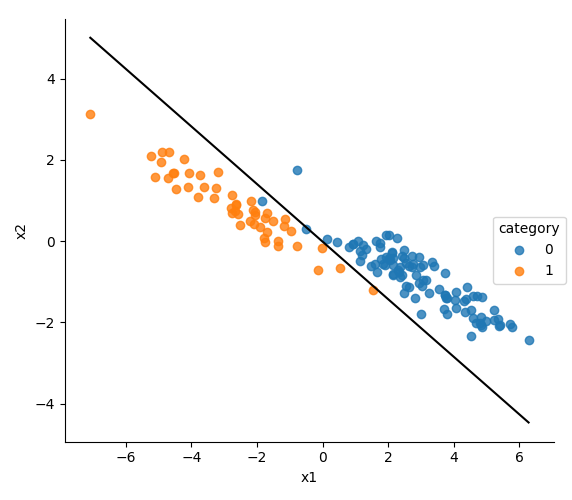
\includegraphics[scale=.45]{a_lda.png}
\end{minipage}
\begin{minipage}{0,45\textwidth}
\caption{IRLS}
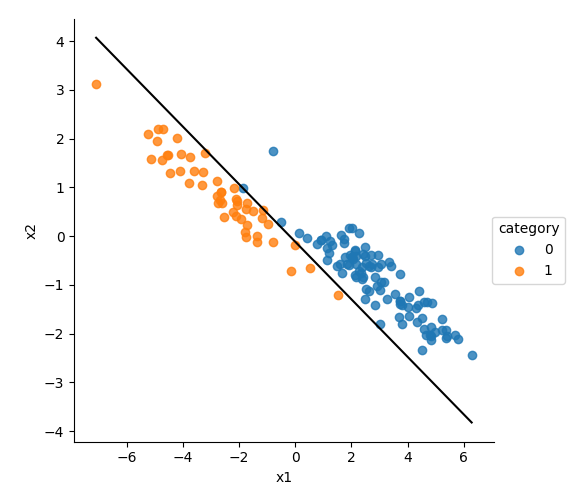
\includegraphics[scale=.45]{a_irls.png}
\end{minipage}
\begin{minipage}{0,45\textwidth}
\caption{Linear Regression}
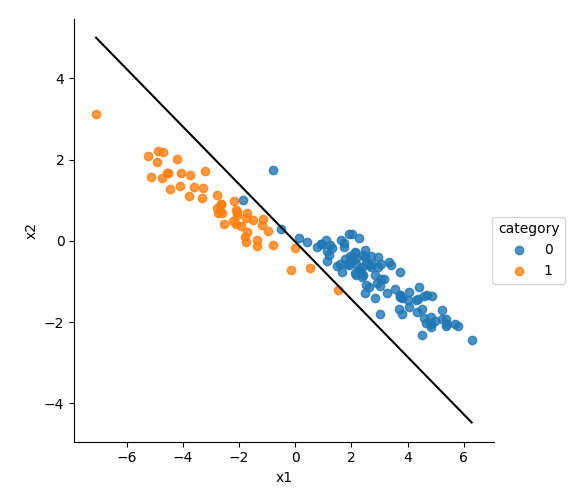
\includegraphics[scale=.45]{a_lr.png}
\end{minipage}
\begin{minipage}{0,45\textwidth}
\caption{QDA}
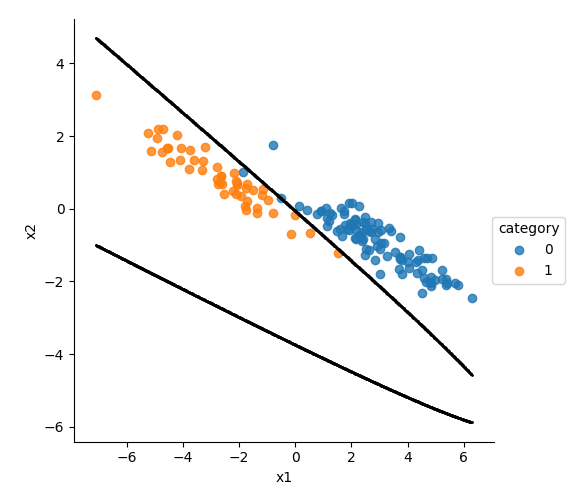
\includegraphics[scale=.45]{a_qda.png}
\end{minipage}
\end{figure}
\begin{minipage}[c]{0,35\textwidth}
Results (\% of success)\\
\begin{tabular}{|c|c|c|}
\hline 
• & Train & Test \\ 
\hline 
LDA & 98.7 & 98.0 \\ 
\hline 
IRLS & 100 & 96.6 \\ 
\hline 
LR & 98.7 & 97.9 \\ 
\hline 
QDA & 99.3 & 98.0 \\ 
\hline 
\end{tabular} 
\end{minipage}
\begin{minipage}{0,6\textwidth}
In this dataset blue points and orange ones looks like they share the same covarience matrix $\Sigma$. This is confirmed by the great results of LDA which has the same success rate in the testing dataset of QDA which waives the equality of $\Sigma_1$ and $\Sigma_2$. IRLS acheived a 100\% success rate in the trainig set but it clearly overfitted on the training sample (it makes the worst score on the testing set). Finally linear regression performs quite well (almost the same results as LDA) which is not a surprise since the two sets are almost linearly separable.
\end{minipage}
\newpage
\section{Dataset B}
\begin{figure}[h]
\centering
\begin{minipage}{0,45\textwidth}
\caption{LDA}
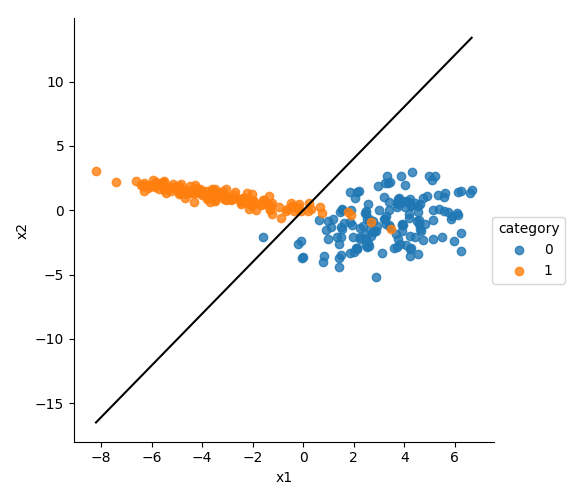
\includegraphics[scale=.45]{b_lda.png}
\end{minipage}
\begin{minipage}{0,45\textwidth}
\caption{IRLS}
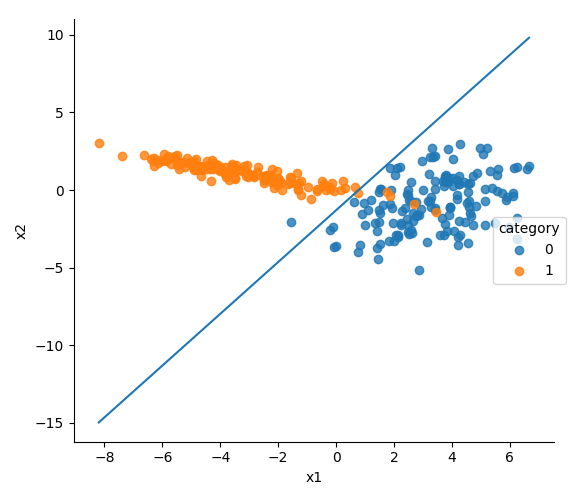
\includegraphics[scale=.45]{b_irls.png}
\end{minipage}
\begin{minipage}{0,45\textwidth}
\caption{Linear Regression}
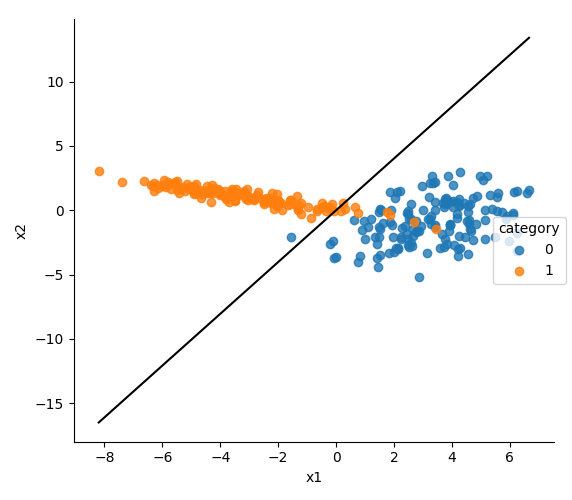
\includegraphics[scale=.45]{b_lr.png}
\end{minipage}
\begin{minipage}{0,45\textwidth}
\caption{QDA}
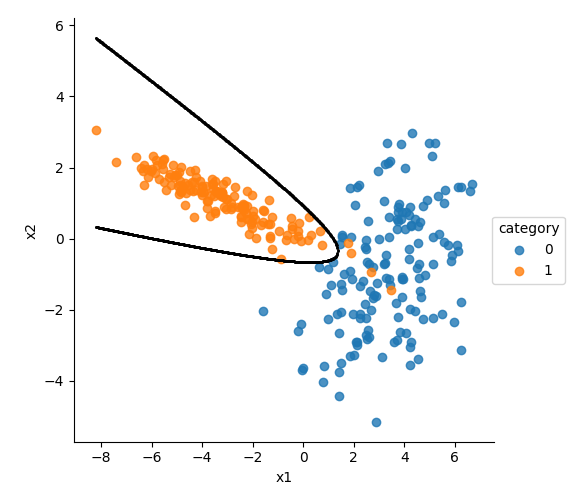
\includegraphics[scale=.45]{b_qda.png}
\end{minipage}
\end{figure}
\begin{minipage}[c]{0,35\textwidth}
Results (\% of success)\\
\begin{tabular}{|c|c|c|}
\hline 
• & Train & Test \\ 
\hline 
LDA & 97.0 & 95.9 \\ 
\hline 
IRLS & 98.0 & 95.7 \\ 
\hline 
LR & 97.0 & 95.9 \\ 
\hline 
QDA & 98.7 & 98.0 \\ 
\hline 
\end{tabular} 
\end{minipage}
\begin{minipage}{0,6\textwidth}
In this dataset, the two distribution doesn't have the same covariance matrix therefore LDA is not the good algorithm to use. However if the two distribution follows indeed a normal distribution with different mean and covariance matrix QDA should perform really well. This assumption is verified by the preformance of QDA (it outperforms the other models). Linear regression and LDA gave the same boundary between both distribution; IRLS returns a shift of that same boundary which provide a better result in training but a worst results than the other two methods in testing.
\end{minipage}
\newpage
\section{Dataset C}
\begin{figure}[h]
\centering
\begin{minipage}{0,45\textwidth}
\caption{LDA}
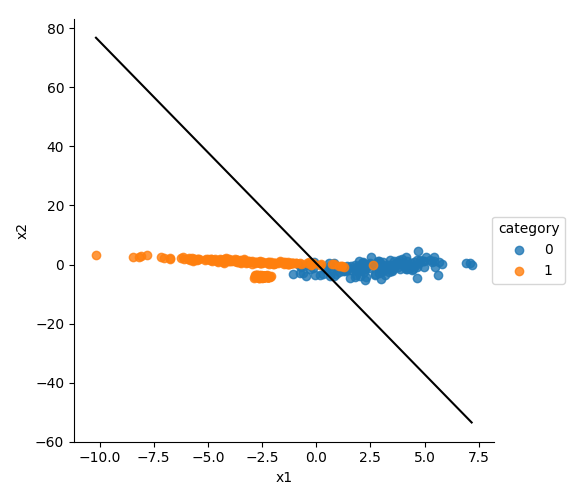
\includegraphics[scale=.45]{c_lda.png}
\end{minipage}
\begin{minipage}{0,45\textwidth}
\caption{IRLS}
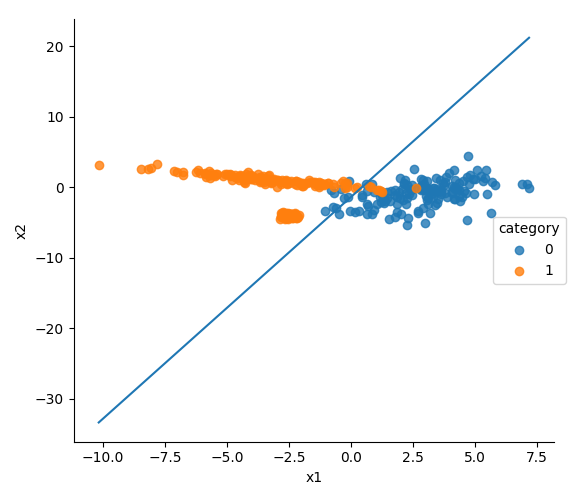
\includegraphics[scale=.45]{c_irls.png}
\end{minipage}
\begin{minipage}{0,45\textwidth}
\caption{Linear Regression}
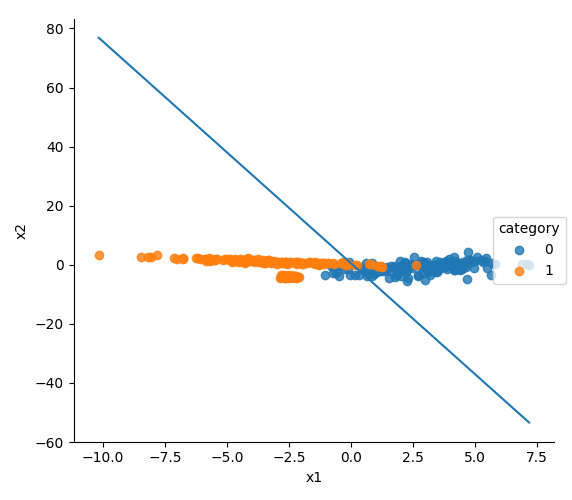
\includegraphics[scale=.45]{c_lr.png}
\end{minipage}
\begin{minipage}{0,45\textwidth}
\caption{QDA}
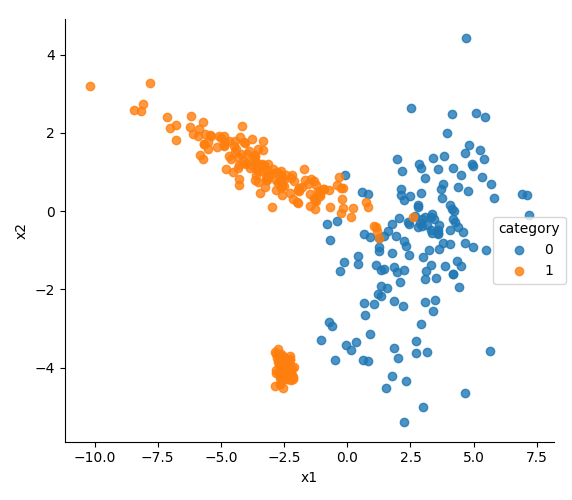
\includegraphics[scale=.45]{c_qda.png}
\end{minipage}
\end{figure}
\begin{minipage}[c]{0,35\textwidth}
Results (\% of success)\\
\begin{tabular}{|c|c|c|}
\hline 
• & Train & Test \\ 
\hline 
LDA & 94.5 & 95.8 \\ 
\hline 
IRLS & 96.0 & 97.7 \\ 
\hline 
LR & 94.5 & 95.8 \\ 
\hline 
QDA & 94.8 & 96.2 \\ 
\hline 
\end{tabular} 
\end{minipage}
\begin{minipage}{0,6\textwidth}
In this dataset the orange distribution doesn't seem to follow a normal distribution because their are two modes. Therefore LDA and QDA eventhough they will provide a good approximation won't be the best option for that task. The two distribution aren't linearly separable; therefore the linear regression won't provide the best results. This leaves us with the logistic regression performed by the IRLS which as a matter of fact outperform the other models and manage to get the generalize surprisingly well the separation of the two distribution (its testing score is higher than its training one).
\end{minipage}
\newpage
\section{Proof}
\subsection{Exercise 1}
We have $N$ samples $(x_i,y_i)$
$\pmb{\pi} = (\pi_1, ..., \pi_M), \pmb{\theta} = (\theta_{1,1}, ... \theta_{M,K})$	\\
$a_m = \mid \{ i \mid  z_i = m, \forall i \in [1,N]\}\mid $, $b_{m,k} = \mid \{ i \mid  z_i = m \text{ and } x_i = k, \forall i \in [1,N]\}\mid $
\begin{align*}
l(\pmb{\pi}, \pmb{\theta}) &= \sum_{i=0}^n log(p(x_i,z_i)) \\
&= \sum_{i=0}^n log(p(x_i \mid  z_i)p(z_i))\\
&= \sum_{i=0}^n (log(\theta_{z_i,x_i}) + log(\pi_{x_i}))
\end{align*}
$l(\pmb{\pi}, \pmb{\theta})$ is concave. We want to minimize $- l(\pmb{\pi}, \pmb{\theta})$ subjected to $\sum_{k=1}^K \pi_k = 1$ and $\sum_{k=1}^K \sum_{m=1}^M \theta_{m,k} = 1$
Lets introduce the langrangian.
$$ L(\pmb{\pi}, \pmb{\theta}, \lambda_1, \lambda_2) = - (\sum_{i=0}^n (log(\theta_{z_i,x_i}) + log(\pi_{x_i}))) + \lambda_1(\sum_{k=1}^K \pi_k - 1) + \lambda_2(\sum_{k=1}^K \sum_{m=1}^M \theta_{m,k} - 1) $$
The Slater’s constraint qualification are trivialy verified and therefore the problem has strong duality property. Therefore we have
$$ \min_{\pmb{\pi}, \pmb{\theta}} - l(\pmb{\pi}, \pmb{\theta}) = \max_{\lambda_1, \lambda_2}  L(\pmb{\pi}, \pmb{\theta}, \lambda_1, \lambda_2) $$
Moreover the lagrangian is convex with respect to $\pmb{\pi}$ and $\pmb{\theta}$
$$ \frac{\partial L}{\partial \pi_m} = 0 \Rightarrow \tilde{\pi}_m = \frac{a_m}{\lambda_1}$$
$$ \frac{\partial L}{\partial \theta_{m,k}} = 0 \Rightarrow \tilde{\theta}_{m,k} = \frac{b_{m,k}}{\lambda_2}$$
Using the constrains we can calculate $\lambda_1, \lambda_2$.
\begin{align*}
\tilde{\pi}_m &= \frac{a_m}{N} \\
\tilde{\theta}_{m,k} &= \frac{b_{m,k}}{N}
\end{align*}

\subsection{Exercise 2}
\subsubsection{Generative model LDA}
We have $N$ samples and $n=\mid \{i, y_i = 0, \forall i \in [1,N]\}\mid $
\begin{align*}
l(\omega,\Sigma,\mu_0,\mu_1) &= \sum_{i=1}^N log (p(x_i,y_i)) \\
&= \sum_{i=1}^N log(p(x_i \mid  y_i)p(y_i))\\
&= \sum_{\substack{i=1,\\ y_i=0}}^N log(p(x_i\mid y_i=0)) + nlog(\omega) +  \sum_{\substack{i=1,\\ y_i=0}}^N log(p(x_i\mid y_i=1)) + (N-n)log(1 - \omega)\\
&= - \frac{Nd}{2}log(2\pi) + \frac{N}{2}log(\mid \Sigma^{-1}\mid)  - \sum_{\substack{i=1,\\ y_i=0}}^N \frac{1}{2}(x_i - \mu_0)^T \Sigma^{-1}(x_i - \mu_0) \\ & - \sum_{\substack{i=1,\\ y_i=1}}^N \frac{1}{2}(x_i - \mu_1)^T \Sigma^{-1}(x_i - \mu_1) + nlog(\omega) + (N-n)log(1 -\omega)
\end{align*}
This log likelyhood is not concave in $(\omega,\Sigma, \mu_0, \mu_1)$. It is concave in $(\omega, \mu_0, \mu_1)$ with $\Sigma$ fixed.
$$ \nabla_{\omega} l = \frac{n}{\omega} - \frac{N - n }{1 - \omega} $$
$ \nabla_{\omega} l = 0 $ gives us :
$$ \tilde{\omega} = \frac{n}{N}$$
Calculating the gradient in $\mu_0$, $\mu_1$ and equalating it to 0 gives us.
\begin{align*}
\tilde{\mu}_0 &= \frac{1}{n} \sum_{\substack{i=1,\\ y_i=0}}^N x_i \\
\tilde{\mu}_1 &= \frac{1}{N-n} \sum_{\substack{i=1,\\ y_i=1}}^N x_i
\end{align*}
Let us now differentiate $l$ w.r.t. $\Sigma^{-1}$.\\ Let $A = \Sigma^{-1}$, $\Sigma_0 = \frac{1}{n} \sum_{\substack{i=1,\\ y_i=0}}^N (x_i - \mu_0)^T(x_i - \mu_0)$, \\$\Sigma_1 = \frac{1}{N-n} \sum_{\substack{i=1,\\ y_i=1}}^N (x_i - \mu_1)^T(x_i - \mu_1)$  \\
We have :
\begin{align*}
l(\omega,\Sigma,\mu_0,\mu_1) = &- \frac{Nd}{2}log(2\pi) + \frac{N}{2}log(\mid \Sigma^{-1}\mid) - \frac{1}{2}\text{Trace}(A(n\Sigma_0 + (N-n)\Sigma_1) \\&+ nlog(\omega) + (N-n)log(1 -\omega)\\
\nabla_{A}l = & \frac{N}{2}A^{-1} - \frac{1}{2}(n\Sigma_0 + (N-n)\Sigma_1)
\end{align*}
Which leads to 
$$ \tilde{\Sigma} = \frac{n}{N}\Sigma_0 + \frac{N-n}{N}\Sigma_1 $$
We have found a unique stationnary point for the likelyhood. To be sure it is a maximum we would have to calculate the Hessian.\\
Now we will calculate the $p(y=1 \mid x)$.
$$p(y=1 \mid x) = \frac{p(x \mid y=1)p(y=1)}{p(x)}$$
\begin{align*}
log(\frac{p(y=1 \mid x)}{p(y=0 \mid x)}) &= log(\frac{1-\omega}{\omega}) - \frac{1}{2}(x - \mu_1)\Sigma^{-1}(x - \mu_1) + \frac{1}{2}(x - \mu_0)\Sigma^{-1}(x - \mu_0) \\
log(\frac{p(y=1 \mid x)}{p(y=0 \mid x)}) &= log(\frac{1-\omega}{\omega}) + \frac{1}{2}(\mu_0^T\Sigma^{-1}\mu_0 - \mu_1^T\Sigma^{-1}\mu_1) + x^T\Sigma^{-1}(\mu_1-\mu_0) \\
p(y=1 \mid x) &= \frac{1}{1+\frac{w}{1-w}\exp{(\frac{1}{2}(\mu_1^T\Sigma^{-1}\mu_1 - \mu_0^T\Sigma^{-1}\mu_0 ))}\exp{(-x^T\Sigma^{-1}(\mu_1-\mu_0))}}
\end{align*}
It is of the form
$$ p(y=1 \mid x) = \frac{1}{1+\exp{(-(x^Ta+\alpha))}} $$
It is the formula of logistic regression

\subsubsection{QDA model}
We have $N$ samples and $n=\mid \{i, y_i = 0, \forall i \in [1,N]\}\mid $
\begin{align*}
l(\omega,\Sigma_0, \Sigma_1, \mu_0,\mu_1) &= \sum_{i=1}^N log (p(x_i,y_i)) \\
&= \sum_{i=1}^N log(p(x_i \mid  y_i)p(y_i))\\
&= \sum_{\substack{i=1,\\ y_i=0}}^N log(p(x_i\mid y_i=0)) + nlog(\omega) +  \sum_{\substack{i=1,\\ y_i=0}}^N log(p(x_i\mid y_i=1)) + (N-n)log(1 - \omega)\\
&= nlog(\omega) - \frac{Nd}{2}log(2\pi) + \frac{n}{2}log(\mid \Sigma_0^{-1}\mid)  - \sum_{\substack{i=1,\\ y_i=0}}^N \frac{1}{2}(x_i - \mu_0)^T \Sigma_0^{-1}(x_i - \mu_0) \\ & + (N-n)log(1 -\omega) + \frac{N-n}{2}log(\mid \Sigma_1^{-1}\mid) - \sum_{\substack{i=1,\\ y_i=1}}^N \frac{1}{2}(x_i - \mu_1)^T \Sigma_1^{-1}(x_i - \mu_1)
\end{align*}
This log likelyhood is not concave in $(\omega,\Sigma_0, \Sigma_1, \mu_0, \mu_1)$. It is concave in $(\omega, \mu_0, \mu_1)$ with $\Sigma_0$ and $\Sigma_1$ fixed. We obtain like in the previous questions.
\begin{align*}
\tilde{\omega} &= \frac{n}{N} \\
\tilde{\mu}_0 &= \frac{1}{n} \sum_{\substack{i=1,\\ y_i=0}}^N x_i \\
\tilde{\mu}_1 &= \frac{1}{N-n} \sum_{\substack{i=1,\\ y_i=1}}^N x_i
\end{align*}
Differentiating $l$ w.r.t. $\Sigma_0^{-1}$ with the rest fixed and equalizing to 0 (and then doing the same with $\Sigma_1^{-1}$) gives us.
\begin{align*}
\tilde{\Sigma}_0 &= \frac{1}{n} \sum_{\substack{i=1,\\ y_i=0}}^N (x_i - \mu_0)^T(x_i - \mu_0) \\
\tilde{\Sigma}_1 &= \frac{1}{N-n} \sum_{\substack{i=1,\\ y_i=1}}^N (x_i - \mu_1)^T(x_i - \mu_1)
\end{align*}
We did not provide the calculations because it is amlost the same as above.
\end{document}